\chapter{Pain-Gain Canvas}

The Pain-Gain Canvas provides a structured overview of the challenges (Pains) faced by stakeholders in the Coffee Chain ERP system and the value additions (Gains) that the system delivers. It helps visualize how the ERP addresses critical operational pain points while creating tangible benefits for management, outlet staff, and customers.

\section*{Purpose of Pain-Gain Analysis}
The Pain-Gain Canvas helps stakeholders:
\begin{itemize}
    \item Identify key operational problems in the current workflow.
    \item Highlight the added value that the ERP system provides.
    \item Guide future enhancements and improvements for the ERP module.
    \item Align ERP functionality with organizational goals and user expectations.
\end{itemize}

\section*{Pains: Operational Challenges}

\begin{itemize}
    \item \textbf{Manual sales tracking across outlets:} Tracking sales individually in multiple locations is error-prone and time-consuming.
    \item \textbf{Menu updates not automatically reflected in sales:} Any changes in the coffee menu need to be manually synchronized with the sales module, leading to discrepancies.
    \item \textbf{Limited visibility into customer leads and engagement:} Without centralized CRM integration, marketing and sales teams lack actionable insights.
    \item \textbf{Difficulty generating consolidated reports:} Management cannot easily access regional or outlet-level performance data.
    \item \textbf{Data entry and pricing errors:} Manual processes increase the likelihood of mistakes affecting revenue.
    \item \textbf{Fragmented CRM data across outlets:} Leads and customer interactions are scattered, reducing the effectiveness of customer engagement strategies.
\end{itemize}

\section*{Gains: Value Additions}

\begin{itemize}
    \item \textbf{Centralized ERP platform:} Integrates outlets, sales, menu, and CRM into a single system for efficiency.
    \item \textbf{Real-time menu updates:} Ensures all sales channels reflect the latest product offerings immediately.
    \item \textbf{Automated reporting dashboards:} Provides management with comprehensive, actionable performance metrics for each outlet and region.
    \item \textbf{Enhanced decision-making:} Managers can make data-driven decisions with accurate and consolidated information.
    \item \textbf{Improved customer engagement:} Centralized CRM allows better tracking of leads and interactions across outlets.
    \item \textbf{Reduced errors via automation:} Minimizes mistakes in pricing, stock management, and sales tracking.
\end{itemize}

\section*{Visual Pain-Gain Canvas}

\begin{figure}[H]
\centering
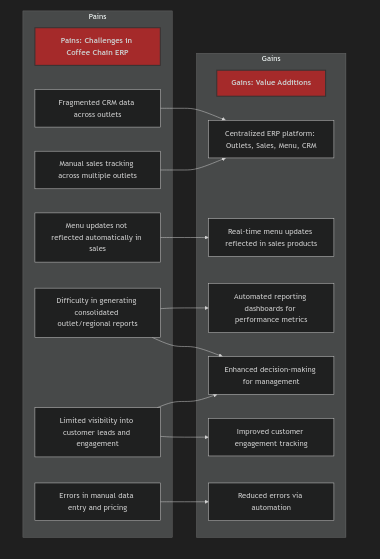
\includegraphics[width=0.85\textwidth,height=0.6\textheight,keepaspectratio]{diagrams/pain_gain.png}
\caption{Pain-Gain Canvas of Coffee Chain ERP}
\end{figure}

\section*{Insights}

\begin{itemize}
    \item The ERP system directly addresses the most critical operational challenges by centralizing processes.
    \item Automated menu updates and reporting dashboards are key features that convert operational pains into tangible gains.
    \item Customer engagement and sales tracking improvements ensure long-term value creation.
    \item The Pain-Gain Canvas serves as a guide for future ERP enhancements, highlighting areas for potential automation and integration.
    \item By addressing operational pains and leveraging system gains, the Coffee Chain ERP ensures:
    \begin{itemize}
        \item Smooth daily operations across all outlets.
        \item Real-time visibility into sales, menu, and CRM data.
        \item Improved decision-making at both outlet and regional levels.
        \item Enhanced customer satisfaction and business efficiency.
    \end{itemize}
\end{itemize}

\subsection*{Strategic Insight}

The Pain-Gain analysis also aligns directly with the Quality Management System (QMS) and the PDCA (Plan-Do-Check-Act) cycle described in Chapter 1.  
By addressing pains through ERP automation and integration, the system supports continuous improvement:

\begin{itemize}
    \item \textbf{Plan:} Identify operational inefficiencies such as manual sales tracking and fragmented CRM data.
    \item \textbf{Do:} Implement ERP features that centralize menu, sales, and CRM into a single platform.
    \item \textbf{Check:} Use automated reporting dashboards to monitor outlet performance, sales trends, and customer engagement.
    \item \textbf{Act:} Refine processes and update system configurations to enhance efficiency and customer satisfaction.
\end{itemize}

This demonstrates that the ERP not only resolves current pains but also creates a framework for sustainable, long-term improvements across the coffee chain.
